% !TEX root = ../thesis-example.tex
%
\chapter{Results}

This chapter will outline the results for both simple and complex models. Ultimately, the difference between our classification of "simple" and "complex" models stems from whether or not the model requires hyperparameters, which must be set before training the model to guide the learning process. The Huber and simple linear regressions are the only two models in our research that do not require this process.

\section{Simple Models}

This section will outline the cross-sectional out-of-sample predictive $R^2$ (denoted by $R^2_{oos}$). We compare eight models which are de (OLS-FF, OLS-3, OLS-5, OLS-7, OLS-15, LR-FF, LR-3, LR-5, LR-7, LR-15). Afterward, we then use the $R^2_{oos}$ to construct statistical learning portfolios and compare overall predictability performance using common statistical, financial metrics. Finally, we selected the best models and assessed the most impactful features for overall performance.

\subsection{Simple out-of-Sample $R^2$ model comparison}

Table (\ref{tab:prediction_sample}) reports the annual $R^2_{oos}$ for the dataset using the simple linear regression and OLS. LR-FF and OLS-FF utilize the Fama-French three-factor model, while LR-3 and OLS-3 utilize the synthetic Fama-French three-factor model. Models such as LR-7, LR-15, OLS-7, and OLS-15 are extensions of the Fama-French three-factor model\footnote{Our Fama-French models use small-minus-big, high-minus-low, the market risk premium, and the three-month treasury bill as its factors. The OLS-3/LR-3 uses 12-month momentum, size, and book-to-market. OLS-7/LR-7 uses OLS-3/LR-3 plus working capital accurals, sales growth, asset growth, and growth in common shareholder equity. OLS-15/LR-15 uses OLS-7/LR-7 plus dividends to price, 36-month momentum, beta, return volatility, share turnover, leverage, and sales to price.}. The final two months, LR-Full and OLS-Full, utilize all of the variables in our dataset. In addition to recording the $R^2_{oos}$ for the entire dataset, we have also recorded the results for the top and bottom 30\% of stocks, based on their market capitalization.

As we can see, the simple linear regression post a lower $R^2_{oos}$ than the Huber regression for all models in our analysis. This should not be surprising, as the Huber regression typically produces a lower $R^2$ due to the way it handles outliers and its objective function, as we've explained in Chapter 4. For the simple linear regression, if the data has outliers, the model may fit these outliers well, which gives a higher $R^2_{oos}$. However, the Huber regression breaks down the influence of these outliers, and the model does not fit them as well, leading to potentially higher residuals. Since our $R^2_{oos}$ depends on residuals, if the model does not fit the outliers well, it may result in a lower $R^2_{oos}$

\begin{table}[ht]\label{tab:oos_simple}
	\centering
	\caption{Annual out-of-sample risk-premium predictive performance ($R^2_{oos}$): simple models}
	\begin{tabular}[t]{lcccccccccc}
		\toprule
		&OLS-FF&OLS-3&OLS-7&OLS-15&OLS-Full&LR-FF&LR-3&LR-7&LR-15&LR-Full\\
		\midrule
		Full Set&2.60&2.85&2.84&2.74&1.79&5.52&6.27&6.26&6.21&5.27\\	
		Top 30\%&3.35&3.86&3.83&3.69&2.85&7.16&7.86&7.84&7.74&6.73\\
		Bottom 30\%&1.51&2.27&2.27&2.17&1.12&4.59&5.35&5.35&5.30&4.28\\			   
		\bottomrule
	\end{tabular}\label{tab:prediction_sample}
\end{table}
\vspace{-7mm}
\begin{figure}[h]
	\centering
	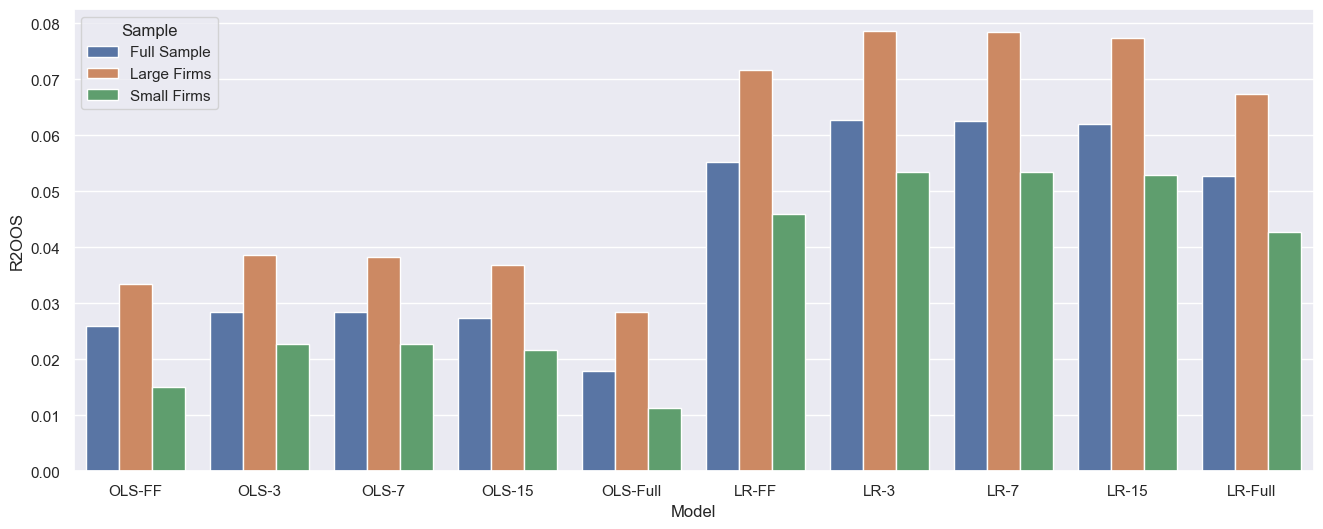
\includegraphics[width=17cm]{content/images/r2_simple}
\end{figure}

As we can also see from the table, the model improves the more factors we introduce; however, we do experience diminishing returns, especially with the simple linear regression. The model peaks in performance with the LR-7, which has an $R^2_{oos}$, but then drops when more features are included. This trait is shared with the Huber regression as well, regardless of the size of the stocks or the focus of the industry in question.

However, recall that we have designated the Fama-French models as our benchmark for our $R^2_{oos}$, which means, at minimum, we expect most models to perform similar, if not better, than our initial benchmark. We can see that most models perform better than the Fama-French models, except for the OLS and LR regression with all the covariates in our dataset.

\subsection{Statistical Learning Portfolios: Simple Models}

After building the simple linear and Huber regressions for each pre-selected portfolio, We construct a statistical learning portfolio by selecting the top 100 stocks with the highest $\hat{y}$. The top 100 stocks are used to generate an equally weighted portfolio, denoted by
\begin{equation}\label{eq:eq_weight}
	r_{p,t}=\frac{1}{100}\sum_{i=1}^{100}r_{i,t}.
\end{equation}

This equally weighted portfolio is generated for each month, $T$, which is then used to compute the average portfolio risk-premium, denoted by
\begin{equation}\label{eq:avg_port_return}
	\bar{r}_p=\frac{1}{T}\sum_{t=1}^{T}r_{t,p}
\end{equation}
This will serve as our basis for analyzing the accuracy and performance of the statistical learning portfolio. The optimal prediction algorithm can precisely predict the actual returns in an out-of-sample setting.
\begin{table}[ht]
	\centering
	\caption{Performance of the statistical learning portfolios}
	\begin{tabular}[t]{lcccc}
		\toprule
		&Actual Returns $\bar{r}_{p}$&Predicted Returns $\hat{\bar{r}}_{p}$&Volatility $\sigma_r$ & Sharpe ratio \\
		\midrule
		LR-FF &-3.54\%	&-4.75\%&3.12\%&-5.28\%\\
		LR-3&-3.19\%	&-4.07\%&2.61\%&-5.40\%  \\
		LR-7&-3.34\%	&-4.01\%&2.62\%&-5.29\%  \\
		LR-15&-3.28\%	&-3.79\%&2.66\%&-4.94\% \\	   
		LR-Full&-3.26\%	&-3.79\%&3.21\%&-4.09\% \\				   
		OLS-FF&-3.54\%	&-4.60\%&3.34\%&-4.77\% \\		
		OLS-3&-3.16\%	&-4.05\%&2.62\%&-5.36\% \\				
		OLS-3&-3.16\%	&-4.05\%&2.62\%&-5.36\% \\
		OLS-7&-3.26\%	&-4.02\%&2.61\%&-5.34\% \\
		OLS-15&-3.30\%	&-3.81\%&2.69\%&-4.90\% \\
		OLS-Full&-3.28\%&-3.79\%&2.66\%&-4.94\% \\		
		\bottomrule
	\end{tabular}\label{tab:portolio_simple}
\end{table}

Table (\ref{tab:portolio_simple}) shows the performance of the statistical learning portfolios specifically for the Huber and simple learning regression. All ten models mentioned in the previous section are outlined, starting from the benchmark models and increasing incrementally to more complex models. The statistical learning portfolios are presented in terms of the algorithm/model of choice, the actual average portfolio returns, $\bar{r}_p$, the predicted average portfolio returns, $\bar{\hat{y}}_p$, the volatility, which is denoted by
\begin{equation}\label{eq:port_vol}
	\sigma_r=\sqrt{\frac{1}{T-1}\sum_{t=1}^{T}\left(r_{t,p}-\bar{r}_p\right)^2}
\end{equation}
and the sharpe ratio, denoted by $\tfrac{\bar{r}_p}{\sigma_r}$.

Recall from Table (\ref{tab:prediction_sample}) that the models with the best $R^2_{oos}$ were the models with the smallest number of features. However, we can see that the models with the least features tend to be the least accurate. Note that both the LR and OLS Fama-French models should generate the same actual return of -3.54\%; however, the Huber regression performs slightly better for the reasons we have outlined earlier.

As we can see, the more covariates we add to the model, the better it performs. The model with the best performance appears to be the OLS-Full, which uses all of the covariates. However, the LR-Full also uses all of the covariance and performs slightly worse but generates a higher Sharpe ratio (the portfolio is riskier but generates a higher return per unit of risk). Regarding predictability and performance, the Linear Regression model with all features performs the best out of the simpler models.
\subsection{Feature Importance: Simple Models}

It should come as no surprise that the more features introduced to linear models, the more their performance deteriorates. This can happen either through overfitting or multicollinearity. Although two models may perform the same (or better), the model with the most significant explanatory power and interpretability is better. We conducted feature importance analysis on the full covariate simple linear and Huber regression to quantify the interpretability.
\begin{figure}[h]\label{fig:feature_simple}
	\centering
	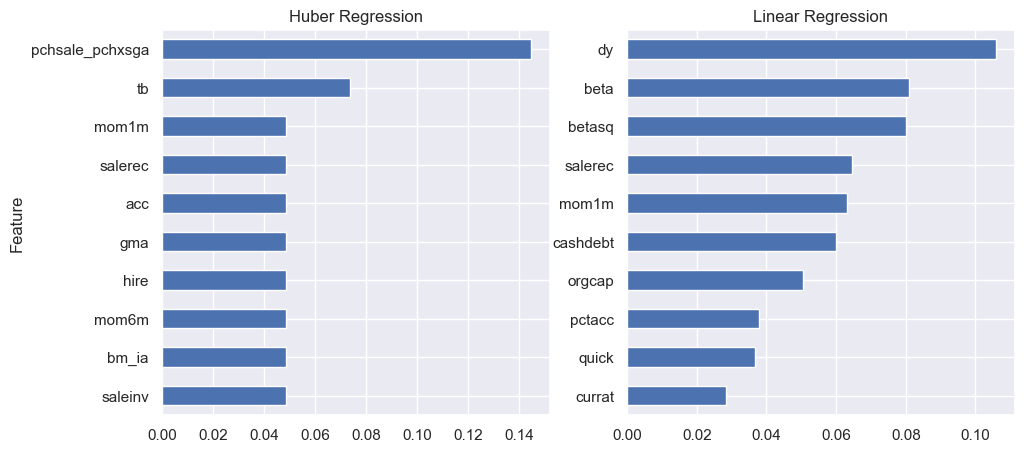
\includegraphics[width=17cm]{content/images/feature_simple}
	\caption{Top 10 important features of the Huber and Simple Linear Regression}
\end{figure}
Feature importance refers to the contribution of each feature variable in a model to predicting the target variable. This can help us identify the most impactful variables, guiding model selection and interpretation. Figure (\ref{fig:feature_simple}) shows the top ten important features for both the Huber and simple linear regression models with all covariates. 

To compute the importance of each feature, we used a five-year training window (2013-2018) and a two-year validation window (2019-2021) to quantify the importance of each feature. This time interval is due to the performance breakdown of many of our statistical learning models within this interval. The process involves training an arbitrary model on the testing set, with the optimal set of hyperparameters, and then making predictions on the validation set, similar to any other machine learning pipeline. Afterward, we ran an algorithm that computes the $R^2$ for each feature individually, which we can use to find the marginal change in the $R^2$ per feature.

This works due to the definition of $R^2$ as $1-RSS/TSS,$ where $\sum\left(y_i-\hat{y}\right)^2$ is the total sum of squares for the response. Since RSS always decreases as more variables are added to the model, the $R^2$ always increases as more variables are added. As such, we can find the variable importance by simply taking the difference in the overall $R^2$ and the marginal $R^2$ per feature.

The simple linear regression model shows that the most important features are dividend to price, beta, beta squared, sales to receivables, 1-month momentum, cash flow to debt, organizational capital, percent accruals, quick ratio, and current ratio. We receive different features regarding what is important for the Huber regression. The most important features for the Huber regression are the percentage change in sales minus the percentage change in SG\&A, tax income to book income, 1-month momentum, sales to receivables, working capital accruals, gross profitability, employee growth rate, 6-month momentum, industry adjusted book to market, and sales to inventory.
\textbf{Add more here potentially}

\section{Complex Models}

This section will outline the cross-sectional out-of-sample predictive $R^2$ (denoted by $R^2_{oos}$). We compare eight models in this section: Elastic Net, Principal Component Regression, Partial Least Squares Regression, and Neural Networks 1-5. Similar to the simple models, we then use the $R^2_{oos}$ to construct statistical learning portfolios, compare overall predictability performance using common statistical and financial metrics, and compare feature importance for the models in each learning category. Finally, we examined how each model adjusts their overall tuning parameters over time, as the respective models change how they learn when more data is introduced to the algorithm.

\subsection{Complex out-of-Sample $R^2$ model comparison}

Compared to the simple models, we receive a wide range of results for complex models. What instantly stands out among the rest is the performance for the principal component regression; when modeling the full dataset, the PCR achieves an $R^2_{oos}$ of 6.12, while all of the other models are under 3\% percent in terms of performance. This may be because, in essence, the PCR does not require any hyperparameter tuning in the same way other models, such as the neural networks and elastic nets. The algorithm decides how many principal components to retain based on cross-validation. Regardless, it is still worth noting that the PCR performs the best out of all cross-sections.

\begin{table}[ht]
	\centering
	\caption{Annual out-of-sample risk-premium predictive performance ($R^2_{oos}$): complex models}
	\begin{tabular}[t]{lccccccccc}
		\toprule
		&ENet&PCR&PLS&GBRT&NN-1&NN-2&NN-3&NN-4&NN-5\\
		\midrule
		Full Set&2.74&6.12&1.82&0.02&1.89&1.90&1.97&1.79&2.06\\	
		Top 30\%&2.42&7.66&3.06&1.06&3.05&2.64&2.83&2.82&2.69\\
		Bottom 30\%&2.54&5.27&2.26&0.09&1.77&1.46&1.54&1.64&1.56\\			   
		\bottomrule
	\end{tabular}\label{tab:prediction_complex}
\end{table}
\vspace{-7mm}
\begin{figure}[h]
	\centering
	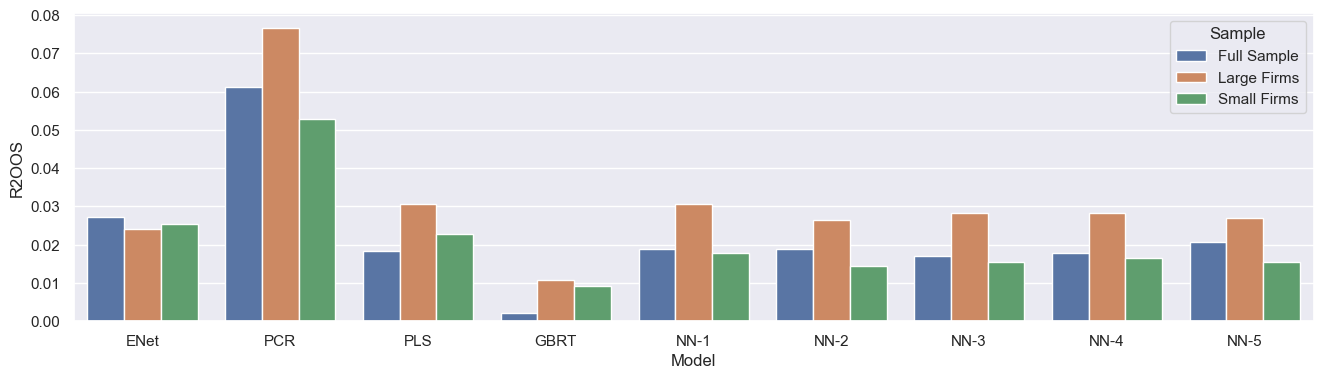
\includegraphics[width=15cm]{content/images/r2_complex}
\end{figure}

The ENet and PLS model performs consistently well. Unfortunately, by far, the model with the worst out-of-sample performance is the Gradient Boosted Regression Trees, despite the limited number of parameters used for training, barely scratching a whole percentage point. This performance is disappointing, considering it's an ensemble model; however, complexity only sometimes ensures better performance or results.

The neural network models perform consistently better based on the number of hidden layers and neurons. The best-performing model in the set is PLS for the full dataset. However, for other cross-sections, the model neural network performs less consistently. This may be due to the lack of available observations in the raw input vector used for each hidden layer.

\subsection{Statistical Learning Portfolios: Complex Models}
Using equations (\ref{eq:eq_weight}), (\ref{eq:avg_port_return}), and (\ref{eq:port_vol}), we derive the output in Table (\ref{tab:portolio_complex}), which shows the performance of statistical learning portfolios for the more complex models. The models that seems to match the actual returns fairly well are the PLS, PCR, ENet and NN-1 models. As expected, the neural network models perform better the more hidden layers and neurons are added to the model. We can see that there is a greater degree of consistency and performance when implementing models with hyperparameters.

\begin{table}[ht]
	\centering
	\caption{Performance of the statistical learning portfolios (Complex Models)}
	\begin{tabular}[t]{lcccc}
		\toprule
		&Actual Returns $\bar{r}_{p}$&Predicted Returns $\hat{\bar{r}}_{p}$&Volatility $\sigma_r$ & Sharpe ratio \\
		\midrule
		Elastic Net &-3.23\%&-3.81\%&2.64\%&-5.00\%\\		
		PLS &-3.31\%&-3.45\%&3.06\%&-3.90\%\\
		PCR &-3.39\%&-3.89\%&2.70\%&-5.00\%\\
		GBRT &-3.57\%&-4.48\%&3.64\%&-4.17\%\\
		NN-1 &-3.40\%&-1.74\%&2.98\%&-2.02\%\\
		NN-2 &-3.43\%&-1.92\%&2.89\%&-2.31\%\\
		NN-3 &-3.48\%&-1.84\%&2.88\%&-2.21\%\\
		NN-4 &-3.46\%&-2.13\%&2.62\%&-2.81\%\\
		NN-5&-3.47\%&-2.74\%&2.37\%&-4.00\%\\
		\bottomrule
	\end{tabular}\label{tab:portolio_complex}
\end{table}
Based on predicted performance compared to actual performance, we would say that the PLS model performs the best compared to the rest of the complex models. However, regarding the financial metrics, NN-2 performs the best on a risk-adjusted basis.

\subsection{Feature Importance: Complex Models}

Figure (\ref{fig:feat_complex}) shows the feature importance for the more complex models. The same process for computing feature importance for the simple models were also implemented for the more complex models.

\begin{figure}[h]\label{fig:feat_complex}
	\centering
	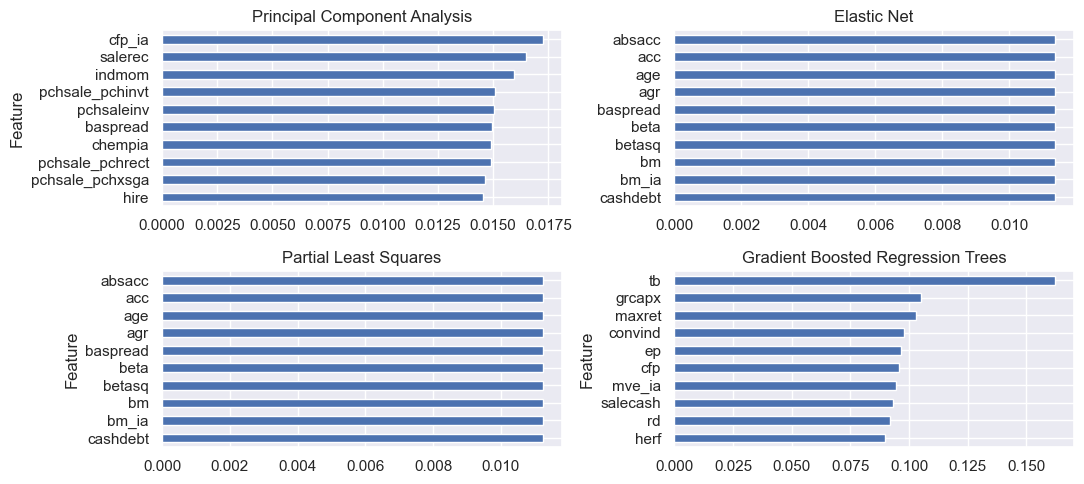
\includegraphics[width=17cm]{content/images/feature_complex}
	\caption{Time-varying model complexity}
\end{figure}

\subsection{Time-Varying Model Complexity}

In order to get a better idea of how our statistical learning models adjust and learn over time, we have conducted a time-varying analysis for PLS, PCR, ENet, and GBRT. The premise behind this analysis is that the complexity of the model is adjusted dynamically over time during the training and evaluation phase. This helps us to improve performance, reduce overfitting, and adapt to the changing distribution of the data.

To conduct this analysis, we merely record the optimal parameters for each rolling window for each machine-learning model in our time interval. Figure (\ref{fig:complexity}) outlines the parameters we have used for the four models in question. For ENet, we recorded the number of coefficients utilized when the L2 parameter, $\lambda$ provided the optimal MSE for each training and validation window; for GBRT, we recorded the max depth for each training and validation window; and for PLS and PCR, we merely recorded the components $K$ that provided the optimal MSE for each training and validation window. The minimum number of components for the PLS and PCR models is 5, while the maximum number of components is 35 and 50, respectively. The highest depth allowed for the GBRT is 2. As always, ENet shrinks the coefficients (potentially to zero) on the shrinkage parameter, $\lambda$, that provides the optimal MSE.

\begin{figure}[h]\label{fig:complexity}
	\centering
	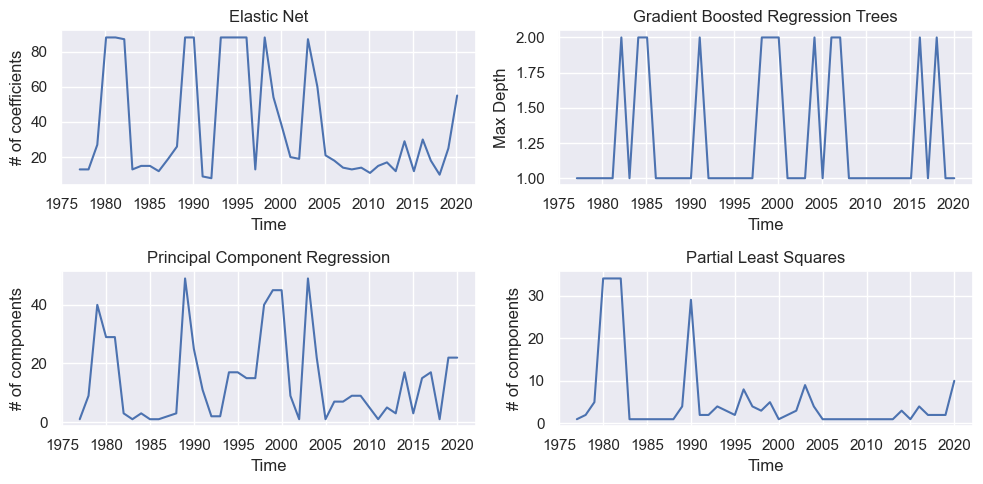
\includegraphics[width=17cm]{content/images/complexity}
	\caption{Time-varying model complexity}
\end{figure}

The time-varying complexity is relatively consistent across the board. From the late 1970s to the early 1980s, from the late 1980s to the early 1990s, from the late 1990s to the early 2000s, in the period of the Financial Crisis, and onward after 2015, the models increase in complexity through these specific eras in the last 45 years. The more features the model requires, the more complex the model becomes.

As the figure above shows, the degree of complexity varies based on the model. For the Elastic Net model, as we can see, when the Lasso penalty $\lambda_1$ dominates, the model becomes more sparse. When the Ridge penalty, $\lambda_2$ dominates, the model increases in complexity and retains the majority of the features in the model. This process occurs until the mid-2010s, where $\sim15-30$ features are retained, and as many as 50 features are retained during the 2020 Pandemic.

A similiar process occurs with the PCR and PLS models, except there is a more significant amount of variation between the complexity based on the time interval. For the PCR, the model used the maximum number of components during the early 1990s and early 2000s, whereas the PLS used the most components in the early 1980s.
\section{Model Selection Overview}
Now, we can compare the best algorithms among the simple and complex models, which leaves us with the simple linear regression, elastic net, partial least square regression, principal component regression, and the neural network with five hidden layers and neurons. Table (\ref{tab:final}) outlines each of these models with the out-of-sample $R^2$ computed for our testing interval.
\begin{table}[ht]
	\centering
	\caption{Performance of the statistical learning portfolios (Complex Models)}
	\begin{tabular}[t]{lccccc}
		\toprule
		&Actual Returns $\bar{r}_{p}$&Predicted Returns $\hat{\bar{r}}_{p}$&Volatility $\sigma_r$ & Sharpe ratio & Out-of-sample $R^2$ \\
		\midrule
		LR-Full&-3.26\%	&-3.79\%&3.21\%&-4.09\%&5.27\% \\	
		Elastic Net &-3.23\%&-3.81\%&2.64\%&-5.00\%&2.74\%\\		
		PLS &-3.31\%&-3.45\%&3.06\%&-3.90\%&1.82\%\\
		PCR &-3.39\%&-3.89\%&2.70\%&-5.00\%&6.12\%\\
		NN-5&-3.47\%&-2.74\%&2.37\%&-4.00\%&2.06\%\\
		\bottomrule
	\end{tabular}\label{tab:final}
\end{table}

If the choice of the machine learning portfolio was based solely on predicted returns, then the $NN-5$ would be the model that generates the better portfolio (although returns are still quite negative). If the same choice was based on the metric of accuracy, then the PLS algorithm generates the best portfolio, as it matches closely to accurate returns. If we made the same choice based on risk or risk-adjusted returns, then the NN-5 would be preferable for investors who were more risk-adverse; however, the PLS generates higher risk-adjusted returns, which is a metric closely monitored by portfolio managers. Finally, we have the matter of predictability, which is where the PCR dominates, followed by the LR-Full.

In choosing the best machine learning portfolio, we feel that it is a goo balance to choose the model with the most accurate performance, with a good risk-adjusted return. The partial least squares is the model that fits this reasonable criteria.

